\appendix
\chapter{Appendix}\label{appendix}
\section{Additional figures and tables}\label{appendix_further_figures}

\begin{figure}[H]
  \centering
  \subfloat{{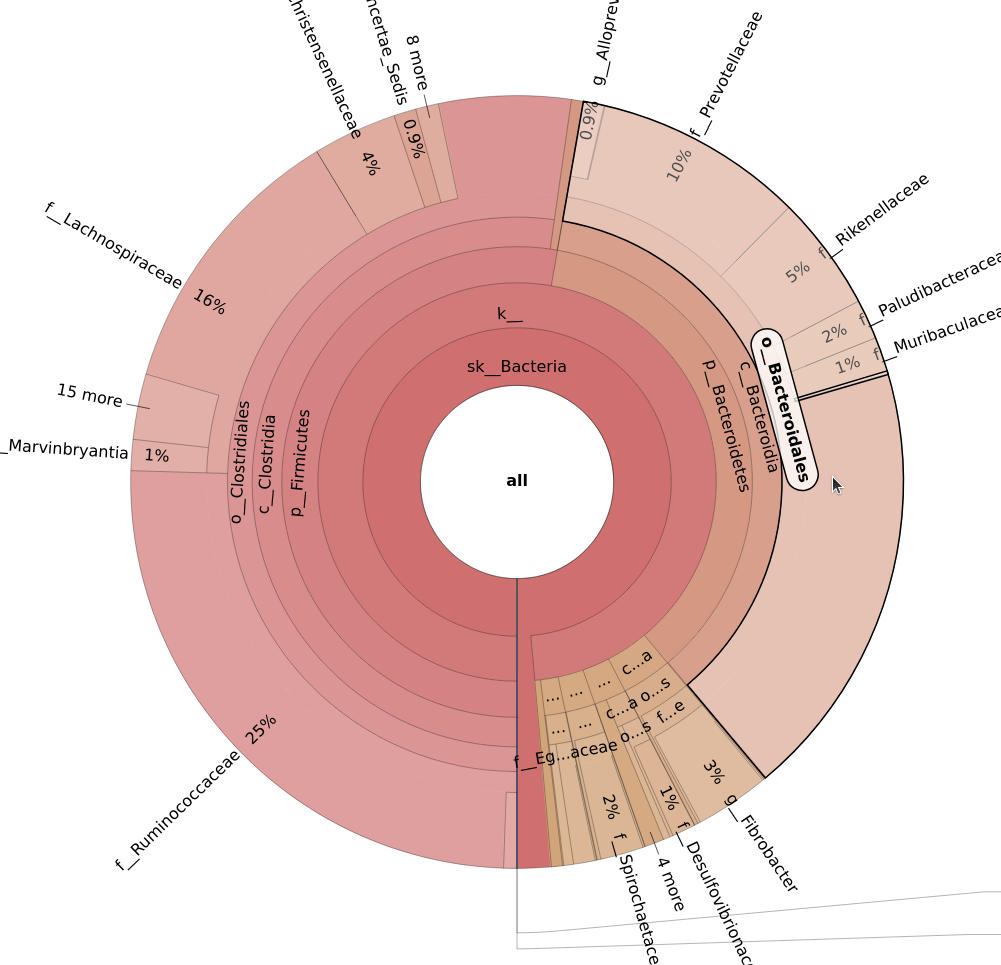
\includegraphics[scale=0.4]{figures/krona_example.png} }}%
  \captionof{figure}[A Krona pie chart example]{\textbf{A Krona pie chart example}. The chart visualizes the taxonomic abundance of the sample ERS4804749 (\Cref{tab:human-gut-samples}).} \label{fig:krona_example}%
\end{figure}

\begin{table}
    \centering
    \begin{tabular}{|c|c|c|}
        \hline
        Species & MGnify & Galaxy\\
        \hline \hline
        Blautia\textunderscore massiliensis & 23 & 16\\
        \hline
        Clostridiales\textunderscore bacterium\textunderscore CHKCI006 & 1 & 1\\
        \hline
        \textbf{Coprococcus\textunderscore catus} & \textbf{1} & \textbf{0}\\
        \hline
        \textbf{Dorea\textunderscore formicigenerans} & \textbf{1} & \textbf{0}\\
        \hline
        Dubosiella\textunderscore newyorkensis & 1 & 1\\
        \hline
        Firmicutes\textunderscore bacterium\textunderscore M10-2 & 1 & 1\\
        \hline
        \textbf{[Clostridium]\textunderscore scindens} & \textbf{1} & \textbf{0}\\
        \hline
        \textbf{Anaerostipes\textunderscore hadrus} & \textbf{0} & \textbf{1}\\
        \hline
        \textbf{Ruminococcus\textunderscore sp} & \textbf{0} & \textbf{1}\\
        \hline
    \end{tabular}
    \caption[Species abundance table for analysis MGYA00566149]{\textbf{Species abundance table for analysis MGYA00566149}. An example of present/absent taxa (see bold marked rows) causing a high Jaccard distance value.}
    \label{jaccard_example}
\end{table}


\subsection{Relative abundance figures}\label{appendix_rel_abundance_figures}

\begin{figure}[H]
  \centering
  \subfloat{{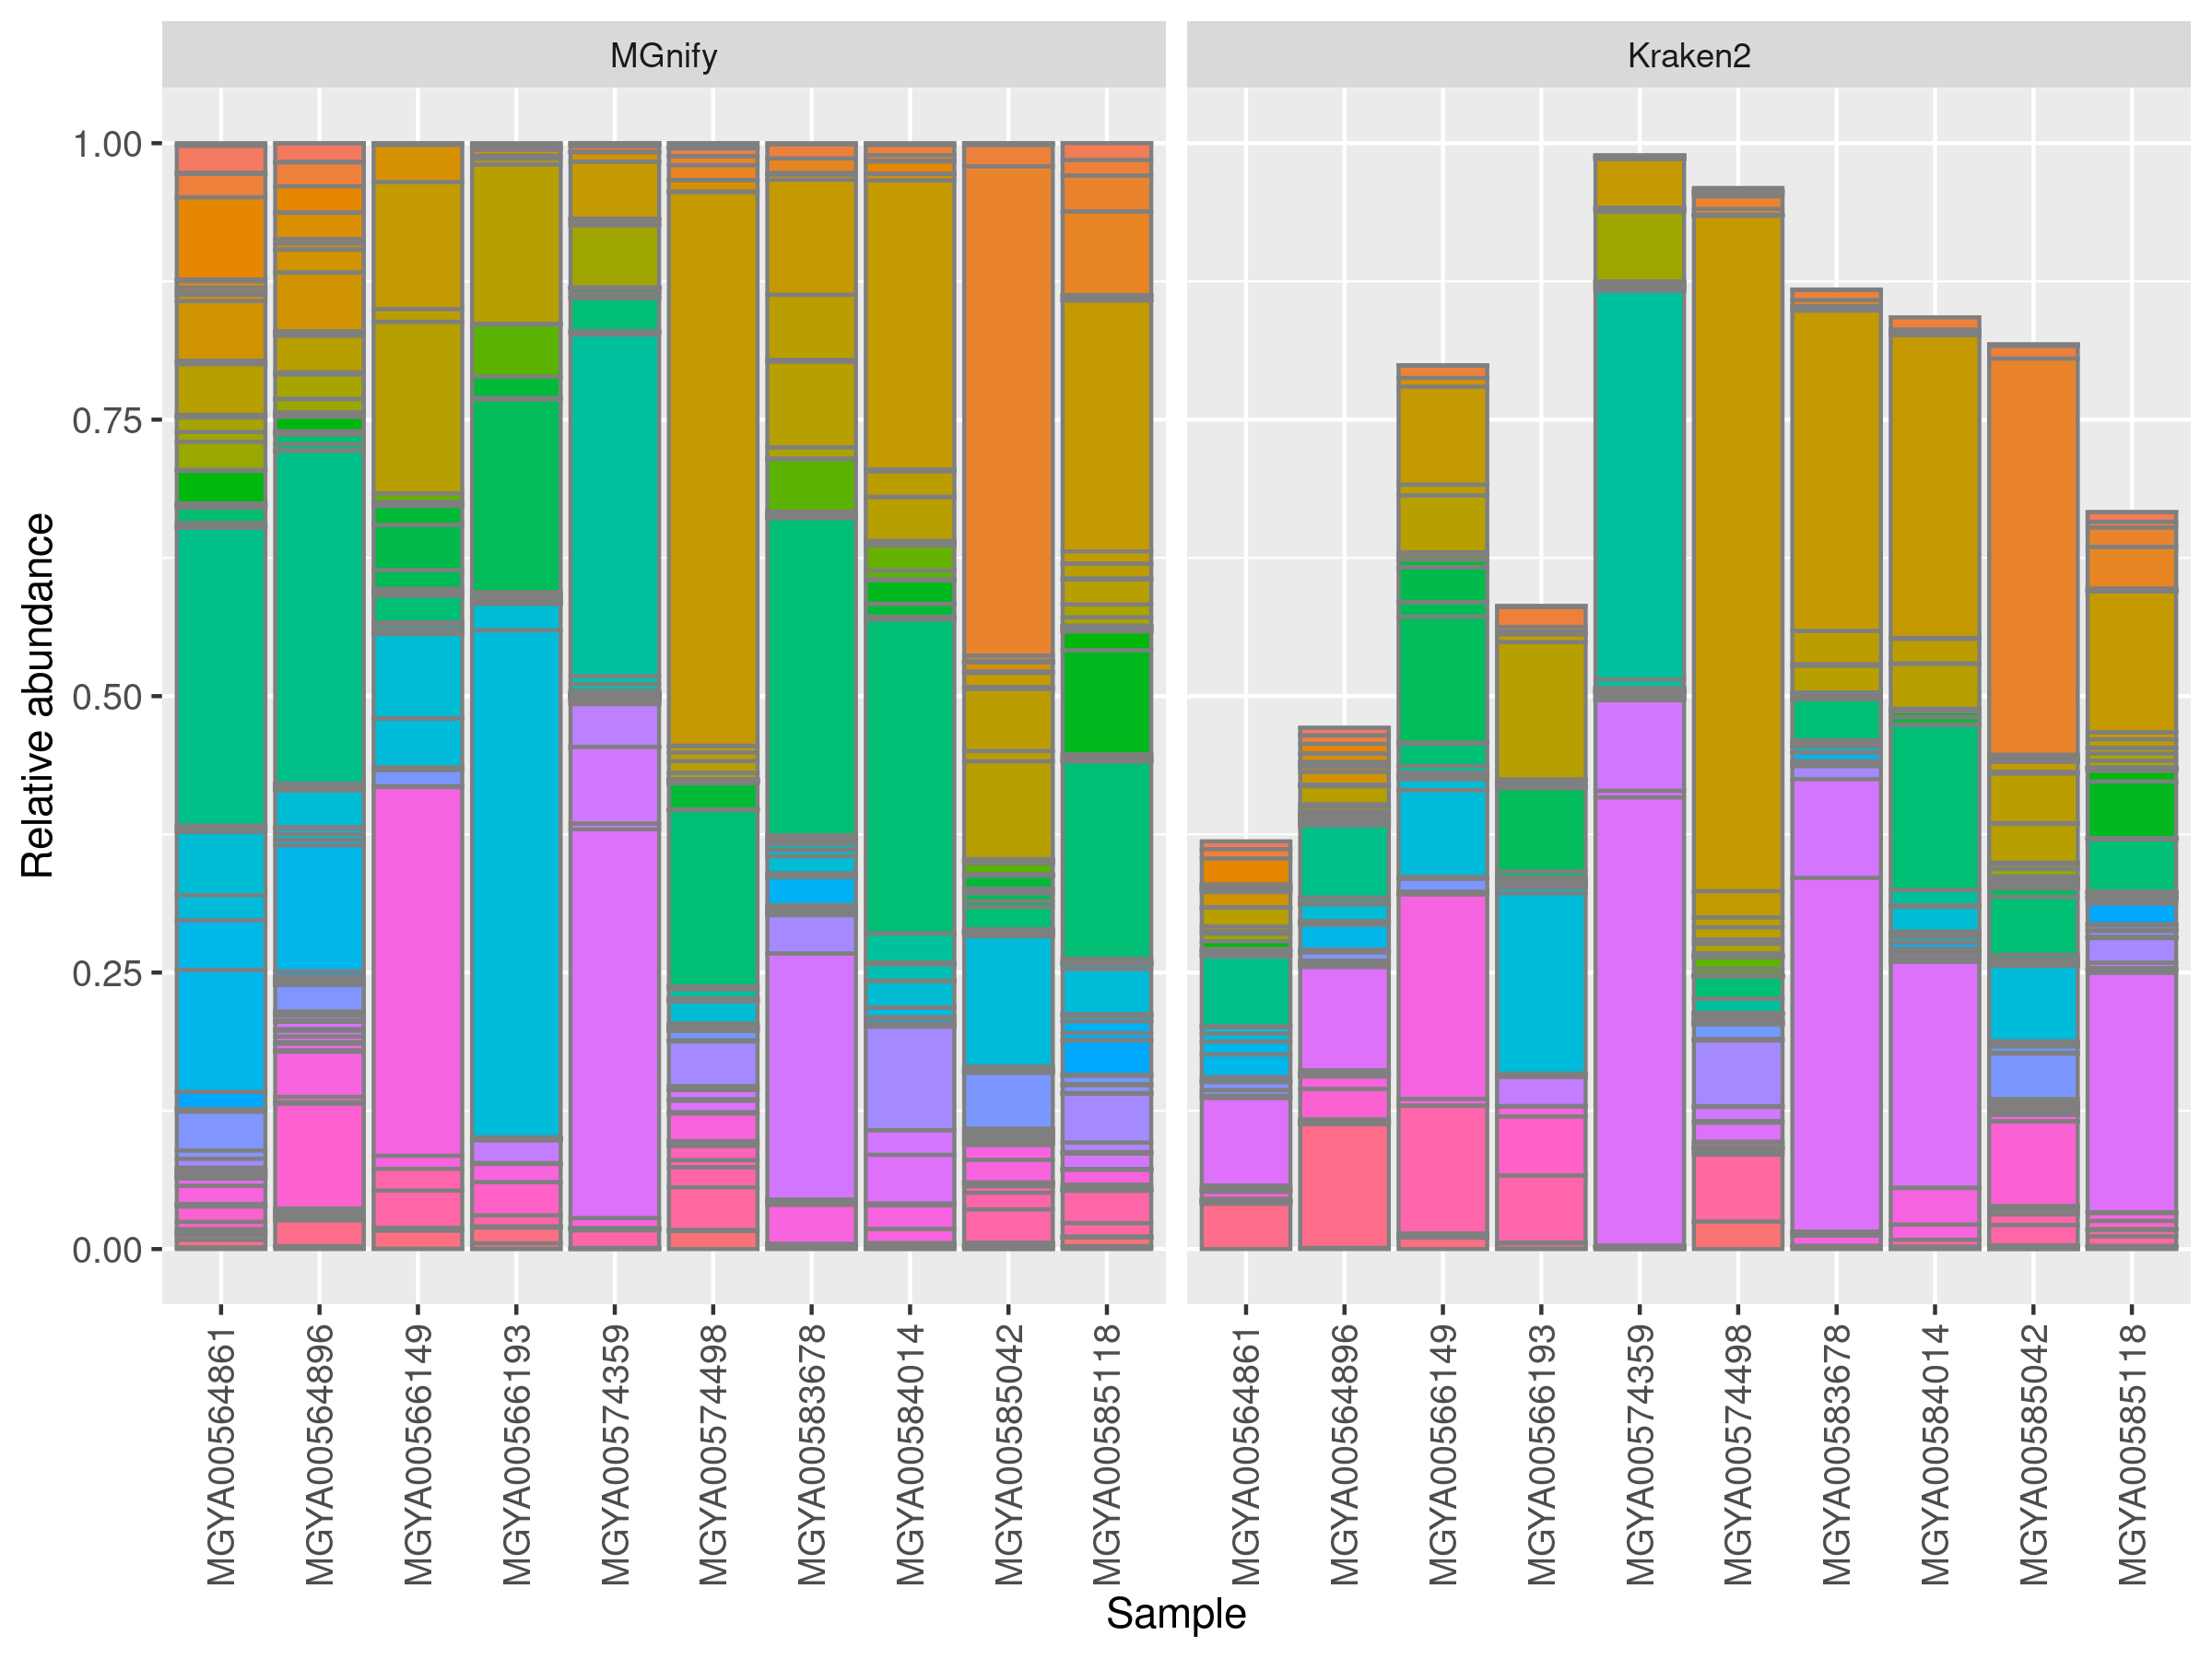
\includegraphics[scale=0.7]{figures/human_gut_abundance_level_g_mgnifyVSKraken.png} }}%
  \captionof{figure}[Differences of relative abundance between MGnify pipeline and Kraken v2 at genus rank for MGnify human large intestine samples]{\textbf{Differences of relative abundance between MGnify pipeline and Kraken v2 at genus rank for MGnify human large intestine samples} (\Cref{tab:human-gut-samples}). Genera that were predicted by Kraken v2 but not present in the MGnify output are not shown. The plot legend can be found in the appendix (\Cref{fig:human_gut_abundance_level_g_mgnifyVSKraken_legend.png})} \label{fig:human_large_intestine_rel_abundance_mgnifyVSkraken2}%
\end{figure}

\begin{figure}[H]
  \centering
  \subfloat{{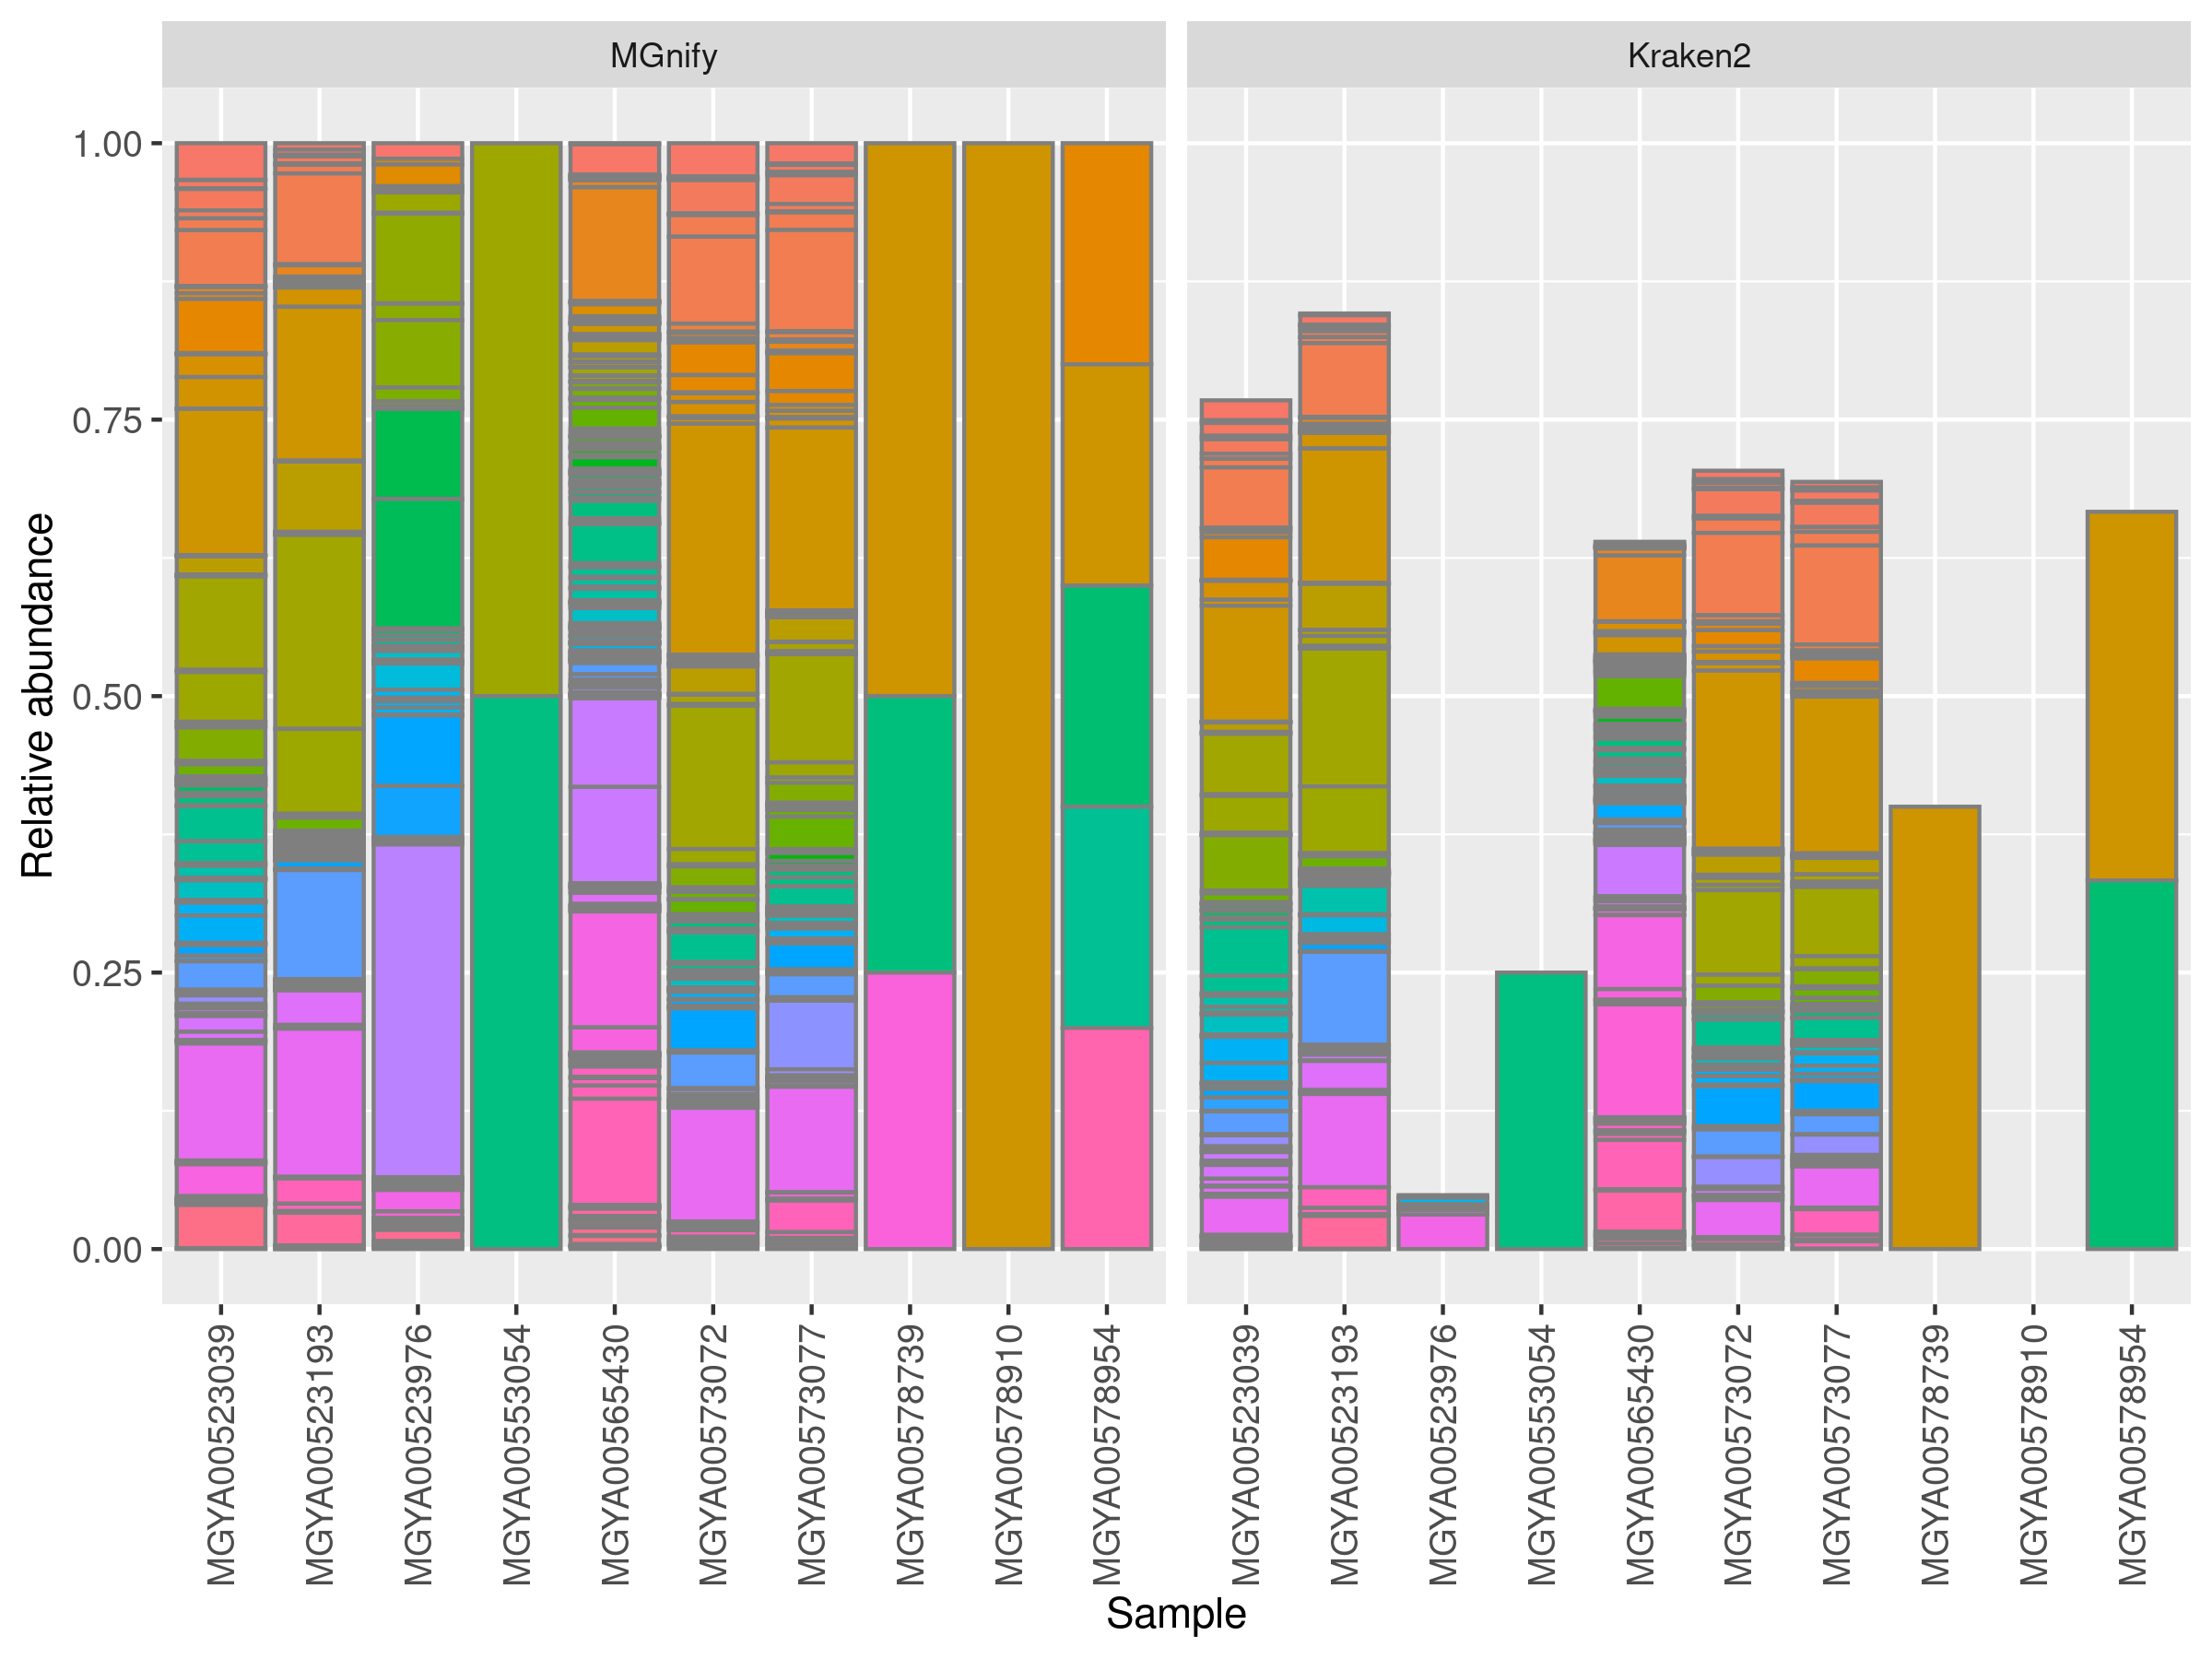
\includegraphics[scale=0.7]{figures/soil_abundance_level_g_mgnifyVSkraken2.png} }}%
  \captionof{figure}[Differences of relative abundance between MGnify pipeline and Kraken v2 at genus rank for MGnify soil samples]{\textbf{Differences of relative abundance between MGnify pipeline and Kraken v2 at genus rank for MGnify soil sample} (\Cref{tab:soil-samples}). Genera that were predicted by Kraken v2 but not present in the MGnify output are not shown. The plot legend can be found in the appendix (\Cref{fig:soil_abundance_level_g_mgnifyVSkraken2_legend.png})} \label{fig:soil_rel_abundance_mgnifyVSkraken2}%
\end{figure}
\newpage

\begin{landscape}
\subsection{Figure legends}\label{appendix_legends}
\vfill
\begin{figure}[H]
  \centering
  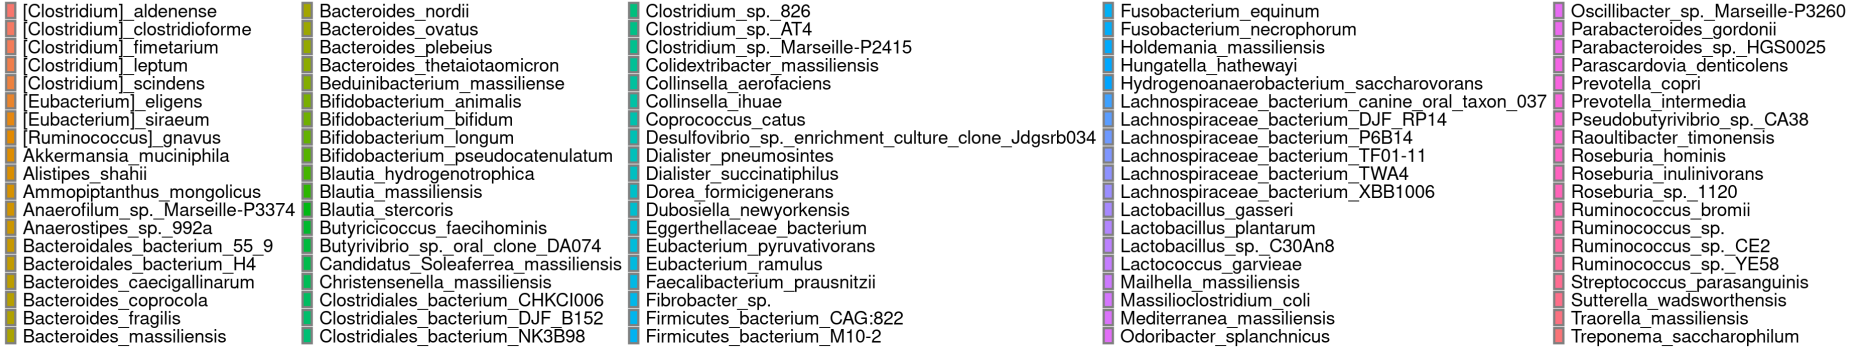
\includegraphics[width=1\linewidth, height=3\textheight, keepaspectratio]{figures/human_gut_abundance_level_s_mgnifyVSgalaxy_legend.png}
  \captionof{figure}[Legend of MGnify human large intestine samples relative abundance plot, comparing MGnify and Galaxy-port at species rank]{\textbf{Legend of MGnify human large intestine samples relative abundance plot, comparing MGnify and Galaxy-port at species rank}.} \label{fig:human_gut_abundance_level_s_mgnifyVSgalaxy_legend.png}%
\end{figure}
\vfill

\begin{figure}
  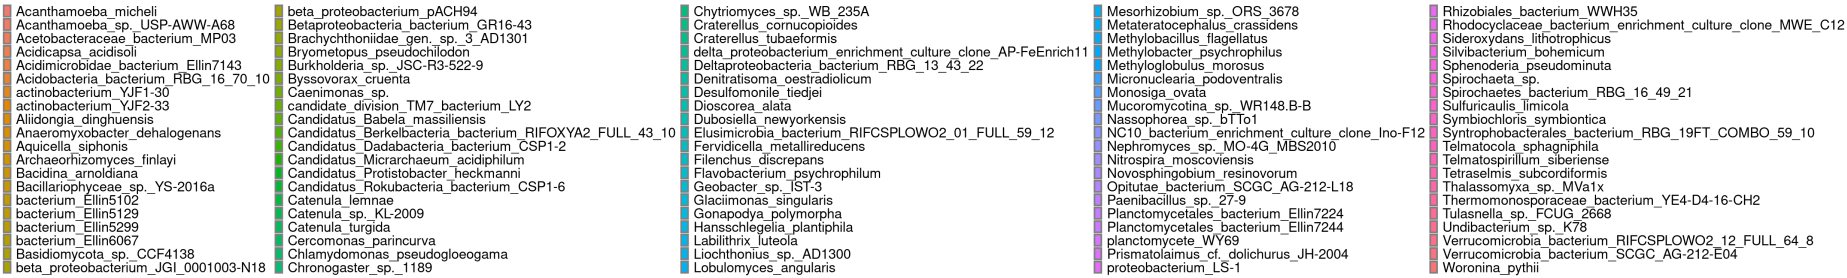
\includegraphics[width=1.1\linewidth, height=0.2\textheight]{figures/soil_abundace_level_s_mgnifyVSgalaxy_legend.png}
  \captionof{figure}[Legend of MGnify soil samples relative abundance plot, comparing MGnify and Galaxy-port at species rank]{\textbf{Legend of MGnify soil samples relative abundance plot, comparing MGnify and Galaxy-port at species rank}.} \label{fig:soil_abundace_level_s_mgnifyVSgalaxy_legend.png}%
\end{figure}
\end{landscape}


\begin{figure}[H]
  \centering
  \subfloat{{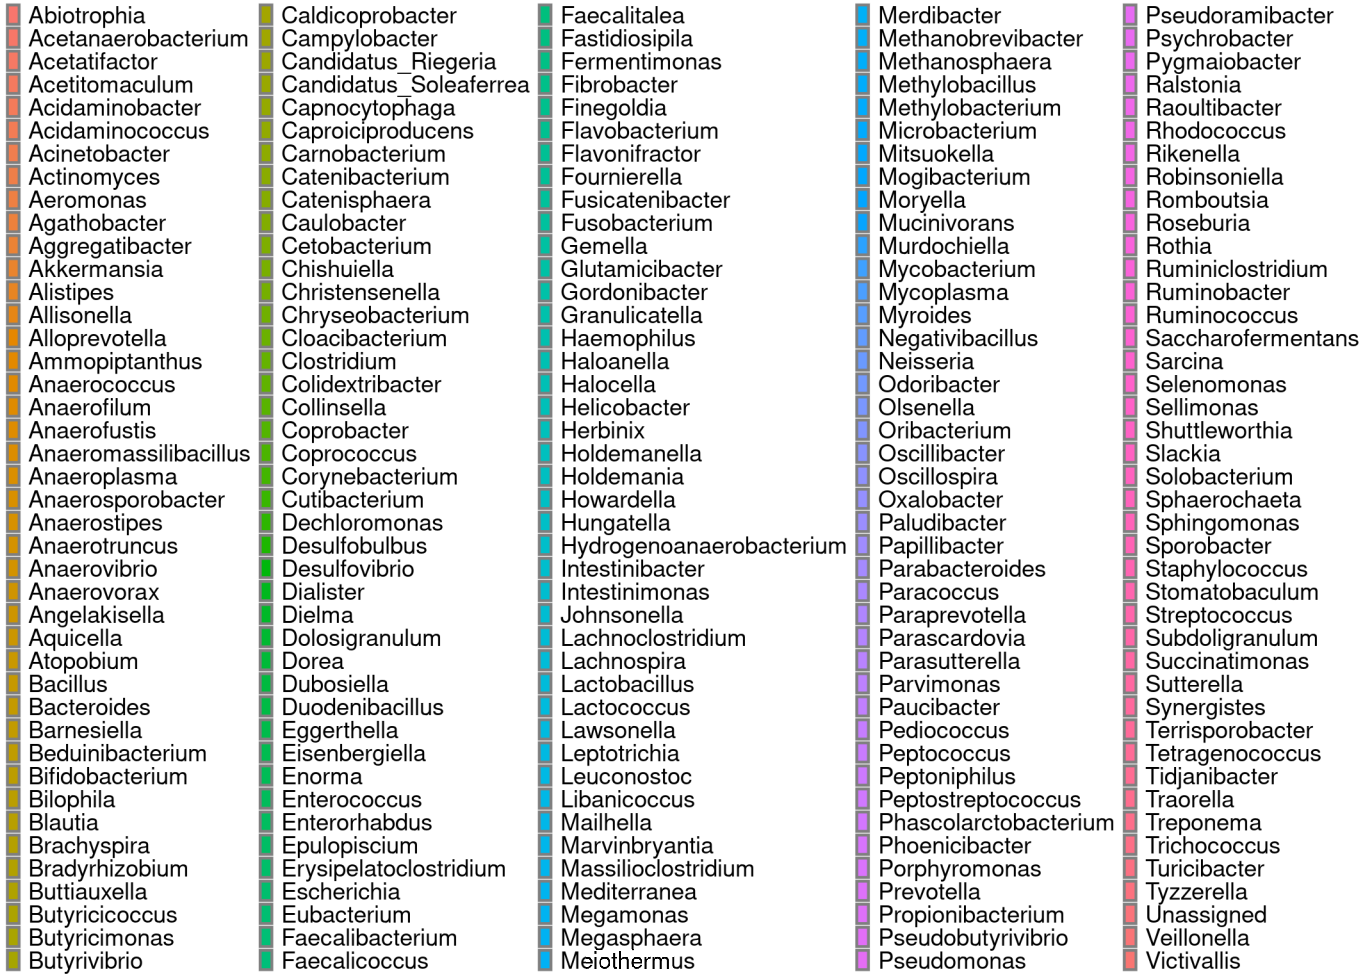
\includegraphics[scale=0.32]{figures/human_gut_abundance_level_g_mgnifyVSgalaxy_legend.png} }}%
  \captionof{figure}[Legend of MGnify human large intestine samples relative abundance plot, comparing MGnify and Galaxy-port at genus rank]{\textbf{Legend of MGnify human large intestine samples relative abundance plot, comparing MGnify and Galaxy-port at genus rank}.} \label{fig:human_gut_abundance_level_g_mgnifyVSgalaxy_legend.png}%
\end{figure}

\begin{figure}[H]
  \centering
  \subfloat{{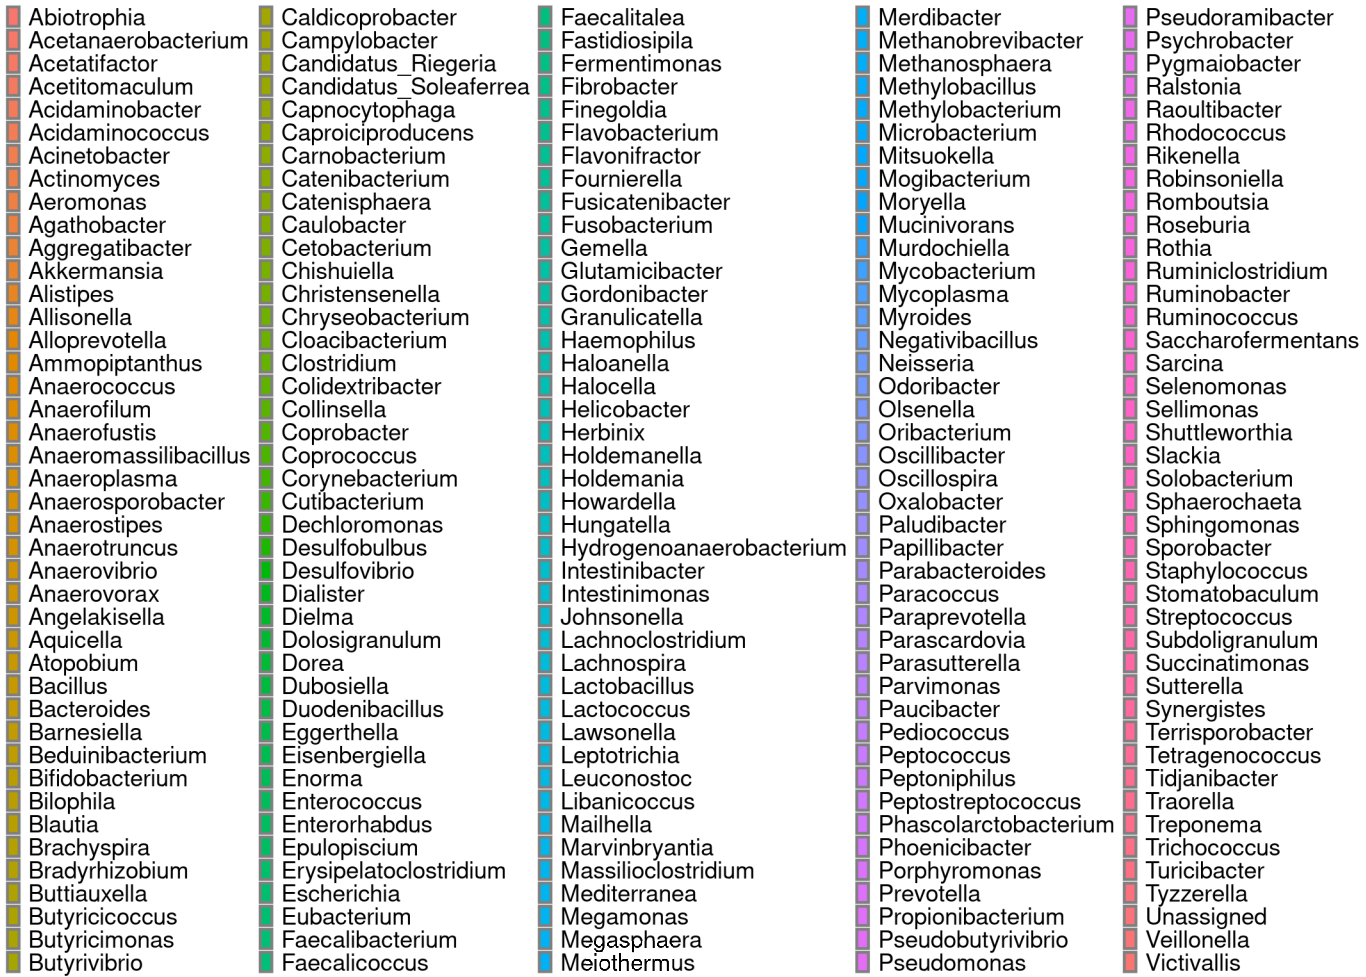
\includegraphics[scale=0.32]{figures/human_gut_abundance_level_g_mgnifyVSKraken_legend.png} }}%
  \captionof{figure}[Legend of MGnify human large intestine samples relative abundance plot, comparing MGnify and Kraken v2 at genus rank]{\textbf{Legend of MGnify human large intestine samples relative abundance plot, comparing MGnify and Kraken v2 at genus rank}.} \label{fig:human_gut_abundance_level_g_mgnifyVSKraken_legend.png}%
\end{figure}

\begin{figure}[H]
  \centering
  \subfloat{{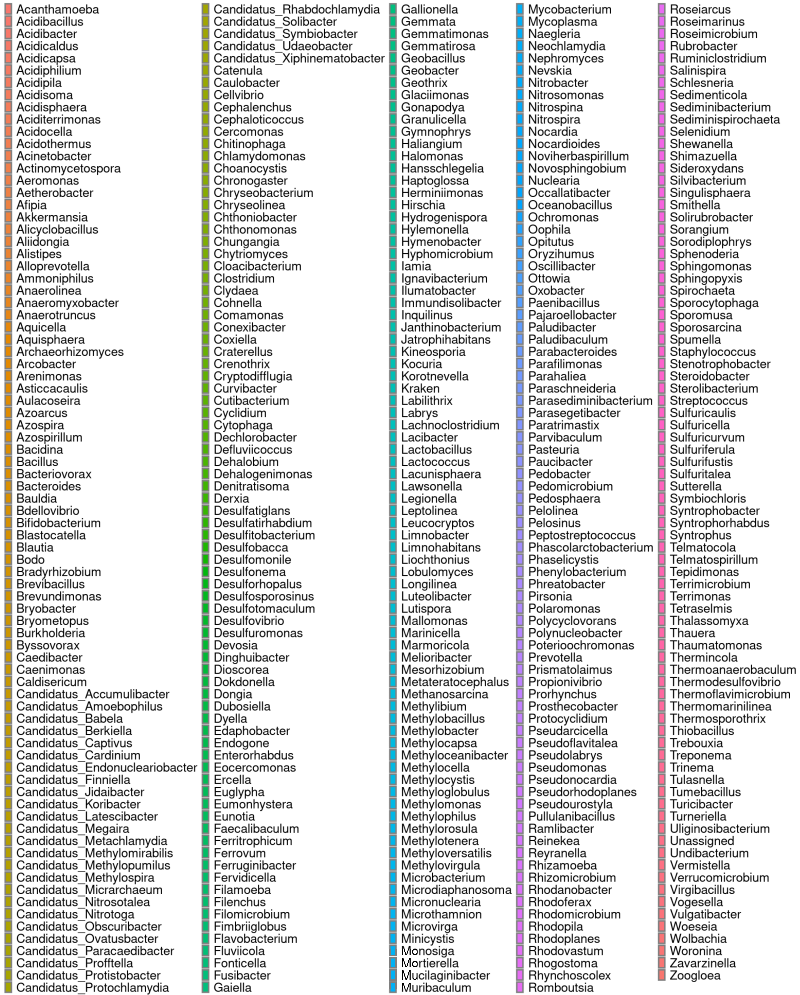
\includegraphics[scale=0.52]{figures/soil_abundance_level_g_mgnifyVSgalaxy_legend.png} }}%
  \captionof{figure}[Legend of MGnify soil samples relative abundance plot, comparing MGnify and Galaxy-port at genus rank]{\textbf{Legend of MGnify soil samples relative abundance plot, comparing MGnify and Galaxy-port at genus rank}.} \label{fig:soil_abundance_level_g_mgnifyVSgalaxy_legend.png}%
\end{figure}

\begin{figure}[H]
  \centering
  \subfloat{{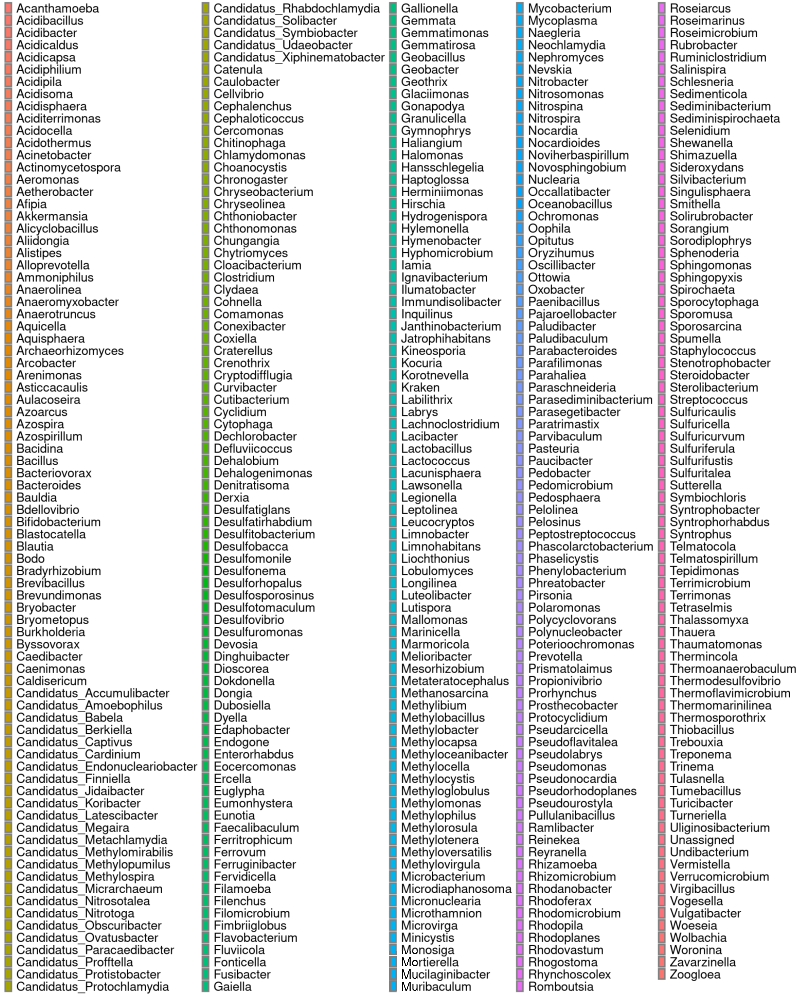
\includegraphics[scale=0.52]{figures/soil_abundance_level_g_mgnifyVSkraken2_legend.png} }}%
  \captionof{figure}[Legend of MGnify soil samples relative abundance plot, comparing MGnify and Kraken v2 at genus rank]{\textbf{Legend of MGnify soil samples relative abundance plot, comparing MGnify and Kraken v2 at genus rank}.} \label{fig:soil_abundance_level_g_mgnifyVSkraken2_legend.png}%
\end{figure}

\begin{figure}[H]
  \centering
  \subfloat{{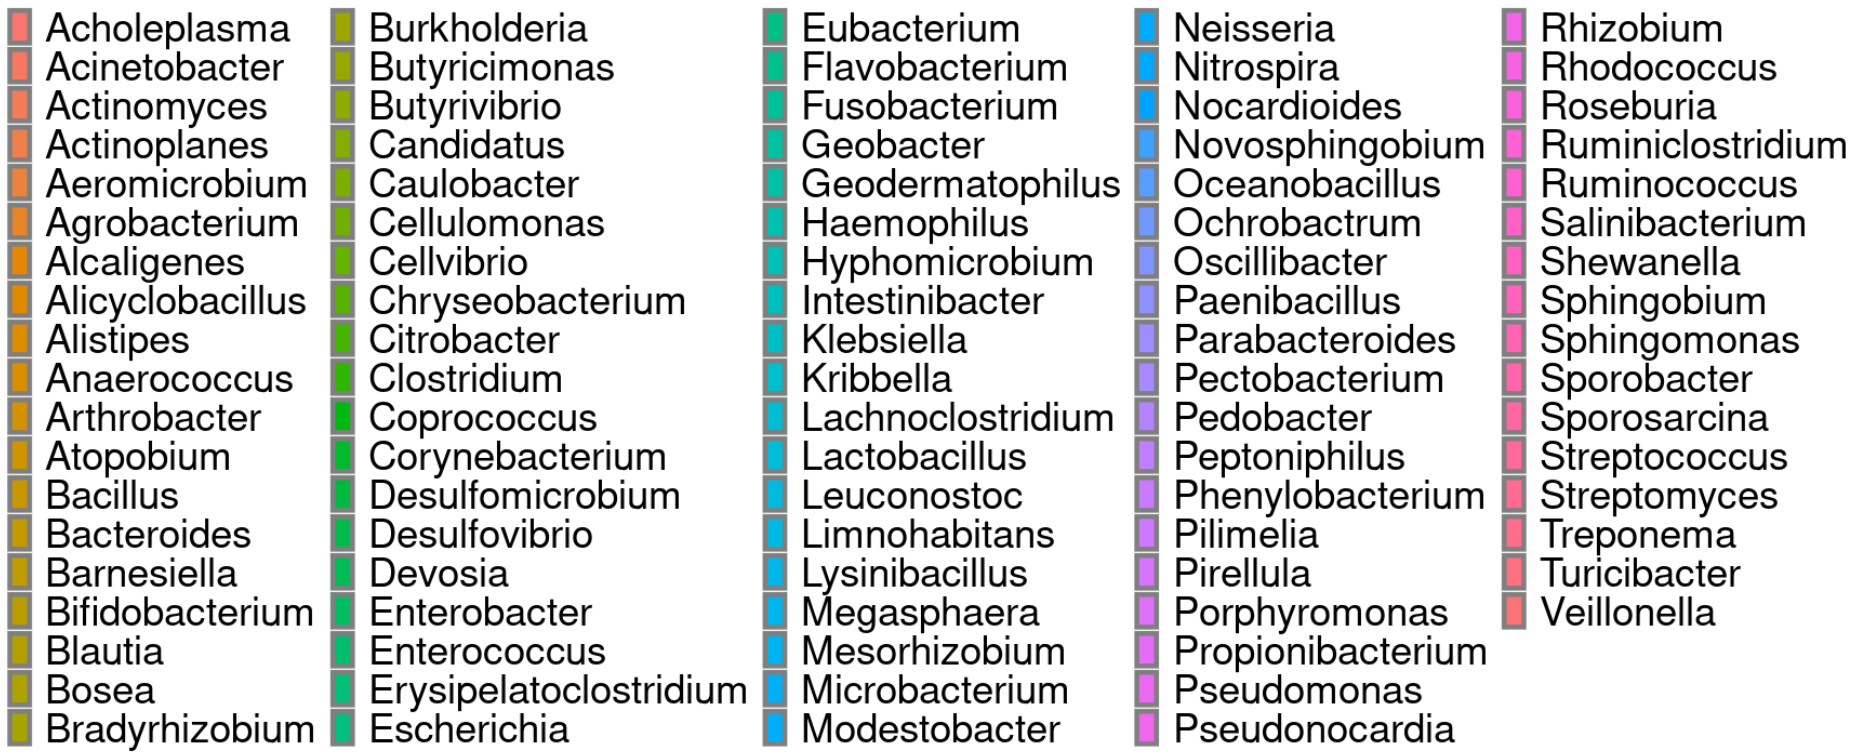
\includegraphics[scale=0.23]{figures/mock_samples_abundance_level_g_legend.png} }}%
  \captionof{figure}[Legend of mock samples relative abundance plot, comparing expected composition, Galaxy-port, and Kraken v2]{\textbf{Legend of mock samples relative abundance plot, comparing expected composition, Galaxy-port, and Kraken v2}.} \label{fig:mock_rel_abundance_level_g_legend}%
\end{figure}

\section{Galaxy workfows}\label{appendix_galaxy_workflows}
\begin{itemize}
    \item rRNA-prediction: \url{https://usegalaxy.eu/u/rz9082/w/rna-prediction}\\
    \item Beta diversity: \url{https://usegalaxy.eu/u/rz9082/w/pairwise-beta-div}
\end{itemize}
\section{Additional software}\label{used_software}
Additional software used during this thesis:
\begin{itemize}
    \item Python v3.7.16, libraries: pandas, seaborn, matplotlib.
    \item R v4.1.2, libraries: ggplot.
\end{itemize}
\section{Results and scripts availability}\label{appendix_results}
All the results obtained and the scripts used for data formatting and visualization during this bachelor thesis are available at: \url{https://drive.google.com/drive/folders/1pgfC_CYVbolskgxhioIXB__449fKtZap}